\documentclass{scrartcl}
\usepackage{cmap}
\usepackage[T1]{fontenc}
\usepackage[utf8]{inputenc}
\usepackage[french]{babel}
\usepackage{microtype}
\usepackage{lmodern}
\usepackage{enumitem}
\usepackage{hyperref}
\usepackage{amsmath, amsthm, amssymb}
\usepackage{booktabs,multirow}
\usepackage{graphicx}
\usepackage{array}

\title{\textbf{Deuxième exemple de document \LaTeX}}
\author{Mon Nom}
\date{\today}

\newtheorem{axiom}{Axiome}


\begin{document}
\maketitle

\section{Mathématiques}
    Une grammaire hors contexte dans l'équation \eqref{equ:grammaire}
    \begin{equation}
        \label{equ:grammaire}
        \begin{aligned}
            S &\rightarrow aS^{'} \\
            S^{'} & \rightarrow bA\\
            A & \rightarrow cA \mid aA' \\
            A^{'} & \rightarrow dB\\
            B & \rightarrow cA \mid aA^{'} \mid b
        \end{aligned}
    \end{equation}

    Utilisons la formule de Stirling qui donne $n! \sim \left(\frac{n}{e}\right)^n \sqrt{2\pi n}$ : 
    \[
    \binom{2n-1}{n-1} = \frac{(2n-1)!}{(n-1)! \cdot n!} = \frac{(2n)!}{2(n!)^2} \sim \frac{\sqrt{4\pi n}\left(\frac{2n}{e}\right)^{2n}}{4\pi n\left(\frac{n}{e}\right)^{2n}} = \frac{2^{2n-1}}{\sqrt{\pi n}} = \Omega(2^n)
    \]
    Ensembles de nombres : $\mathbb{N} \subsetneq \mathbb{Z} \subsetneq \mathbb{D} \subsetneq \mathbb{Q} \subsetneq \mathbb{R} \subsetneq \mathbb{C}$\\
    Formule logique : $\forall \vec{x}\,\phi(\vec{x}) \rightarrow \exists \vec{y}\,\psi(\vec{x}, \vec{y})$.

    \begin{axiom}
        Il existe une unique droite passant par un point parallèle à une droite donnée.
    \end{axiom}
    \begin{proof}
        On ne prouve pas un axiome !
    \end{proof}


\section{Tableaux et figures}
    Voici une description des liens des réseaux sociaux :
    \begin{center}
        \begin{tabular}{cccc}
            \toprule
            {}&{}&\multicolumn{2}{c}{\textbf{Lien Implicite}}\\
            \cmidrule{3-4}
            {}&{}& \textbf{Oui}&\textbf{Non}\\
            \cmidrule{3-4}
            \multirow{2}{*}{\textbf{Lien explicite}} & \textbf{Oui} & Lien agglutinant existant & Lien reliant existant\\
            & \textbf{Non} & Lien agglutinant potentiel & Lien reliant potentiel\\
            \bottomrule
        \end{tabular}        
    \end{center}
    Regardez le beau lapin-canard\footnote{Téléchargé depuis \url{http://commons.wikimedia.org/wiki/File:Duck-Rabbit_illusion.jpg}} de la Figure\ref{fig : lapin-canard} : 
    \begin{figure}
        \centering
        \begin{tabular}{m{.5\linewidth}m{.5\linewidth}}
            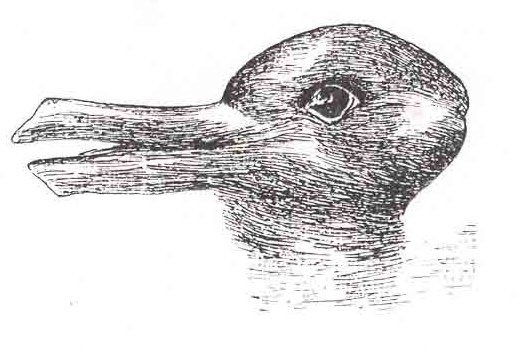
\includegraphics{Duck-Rabbit_illusion.jpg} & Coin ! Ce texte est mis à droite du canard-lapin grâce à un tableau dont chaque case fait .5\texttt{\textbackslash linewidth}
        \end{tabular}
        \caption{Un lapin-canard}        
        \label{fig : lapin-canard}
    \end{figure}

    \begin{table}[h]
        \centering
        \caption{Nombre d'erreurs}
        \begin{tabular}{ccc}
            \toprule
            {} & {Nombre d'erreurs} & {Nombre d'erreurs} \\
            {} & {(cas 1)} & {(cas 2)}\\
            \midrule
            A & 11 & 6\\
            B & 12 & 6\\
            C & 78 & 77\\
            D & 6 & 6\\
            E & 7 & 6\\
            F & 0 & 0\\
            \bottomrule            
        \end{tabular}
    \end{table}

\end{document}

